
\noindent\begin{minipage}{\textwidth}
    \begin{table}[H]
        \centering
        \caption{Hiperparâmetros e Resultados do Melhor Modelo - efficientnet\_v9\_AM\_opt\_aug}
        \vspace{0.2cm}
        \resizebox{\textwidth}{!}{%
            \begin{tabular}{ll | lrrr}
                \hline
                \multicolumn{2}{c|}{\textbf{Hiperparâmetros}} & \multicolumn{4}{c}{\textbf{Métricas por Classe}} \\ \hline
                \textbf{Parâmetro} & \textbf{Valor} & \textbf{Classe} & \textbf{Precisão} & \textbf{Recall} & \textbf{F1-Score} \\ \hline
    Agendador (\$T\_0\$) & 15 & 31.2 & 0,4840 & 0,8717 & 0,6224 \\ 
Agendador de LR & CosineAnnealingWarmRestarts & 31.3 & 0,6056 & 0,4257 & 0,5000 \\ 
Architecture & efficientnet\_b0 & 31.4 & 0,5230 & 0,4333 & 0,4740 \\ 
Batch Size & 32 & 32.3 & 0,7754 & 0,5459 & 0,6407 \\ 
Data Augmentation & False & 32.4 & 0,4902 & 0,4310 & 0,4587 \\ 
Decaimento de Peso (WD) & 0,0001 & 33.3 & 0,6023 & 0,5492 & 0,5745 \\ 
Dropout & 0,3508 & 41.4 & 0,4242 & 0,3182 & 0,3636 \\ 
Função de Perda & CrossEntropyLoss & 41.5 & 0,5769 & 0,7692 & 0,6593 \\ 
Hidden Units & 256 & 42.4 & 0,7381 & 0,4559 & 0,5636 \\ 
Label Smoothing & 0,1000 & 44.4 & 0,5000 & 0,8621 & 0,6329 \\ 
\cline{3-6} 
Otimizador & AdamW & \textbf{Média (Macro)} & 0,6424 & 0,6001 & 0,6084 \\ 
Taxa de Aprendizado (LR) & 8,78e-04 & \textbf{MCC} & \multicolumn{3}{c}{0,5582} \\ 
Unfreeze Layers & 7 &  & & &  \\ 
            \hline
            \end{tabular}%
        }
    \end{table}

    \begin{figure}[H]
        \centering
        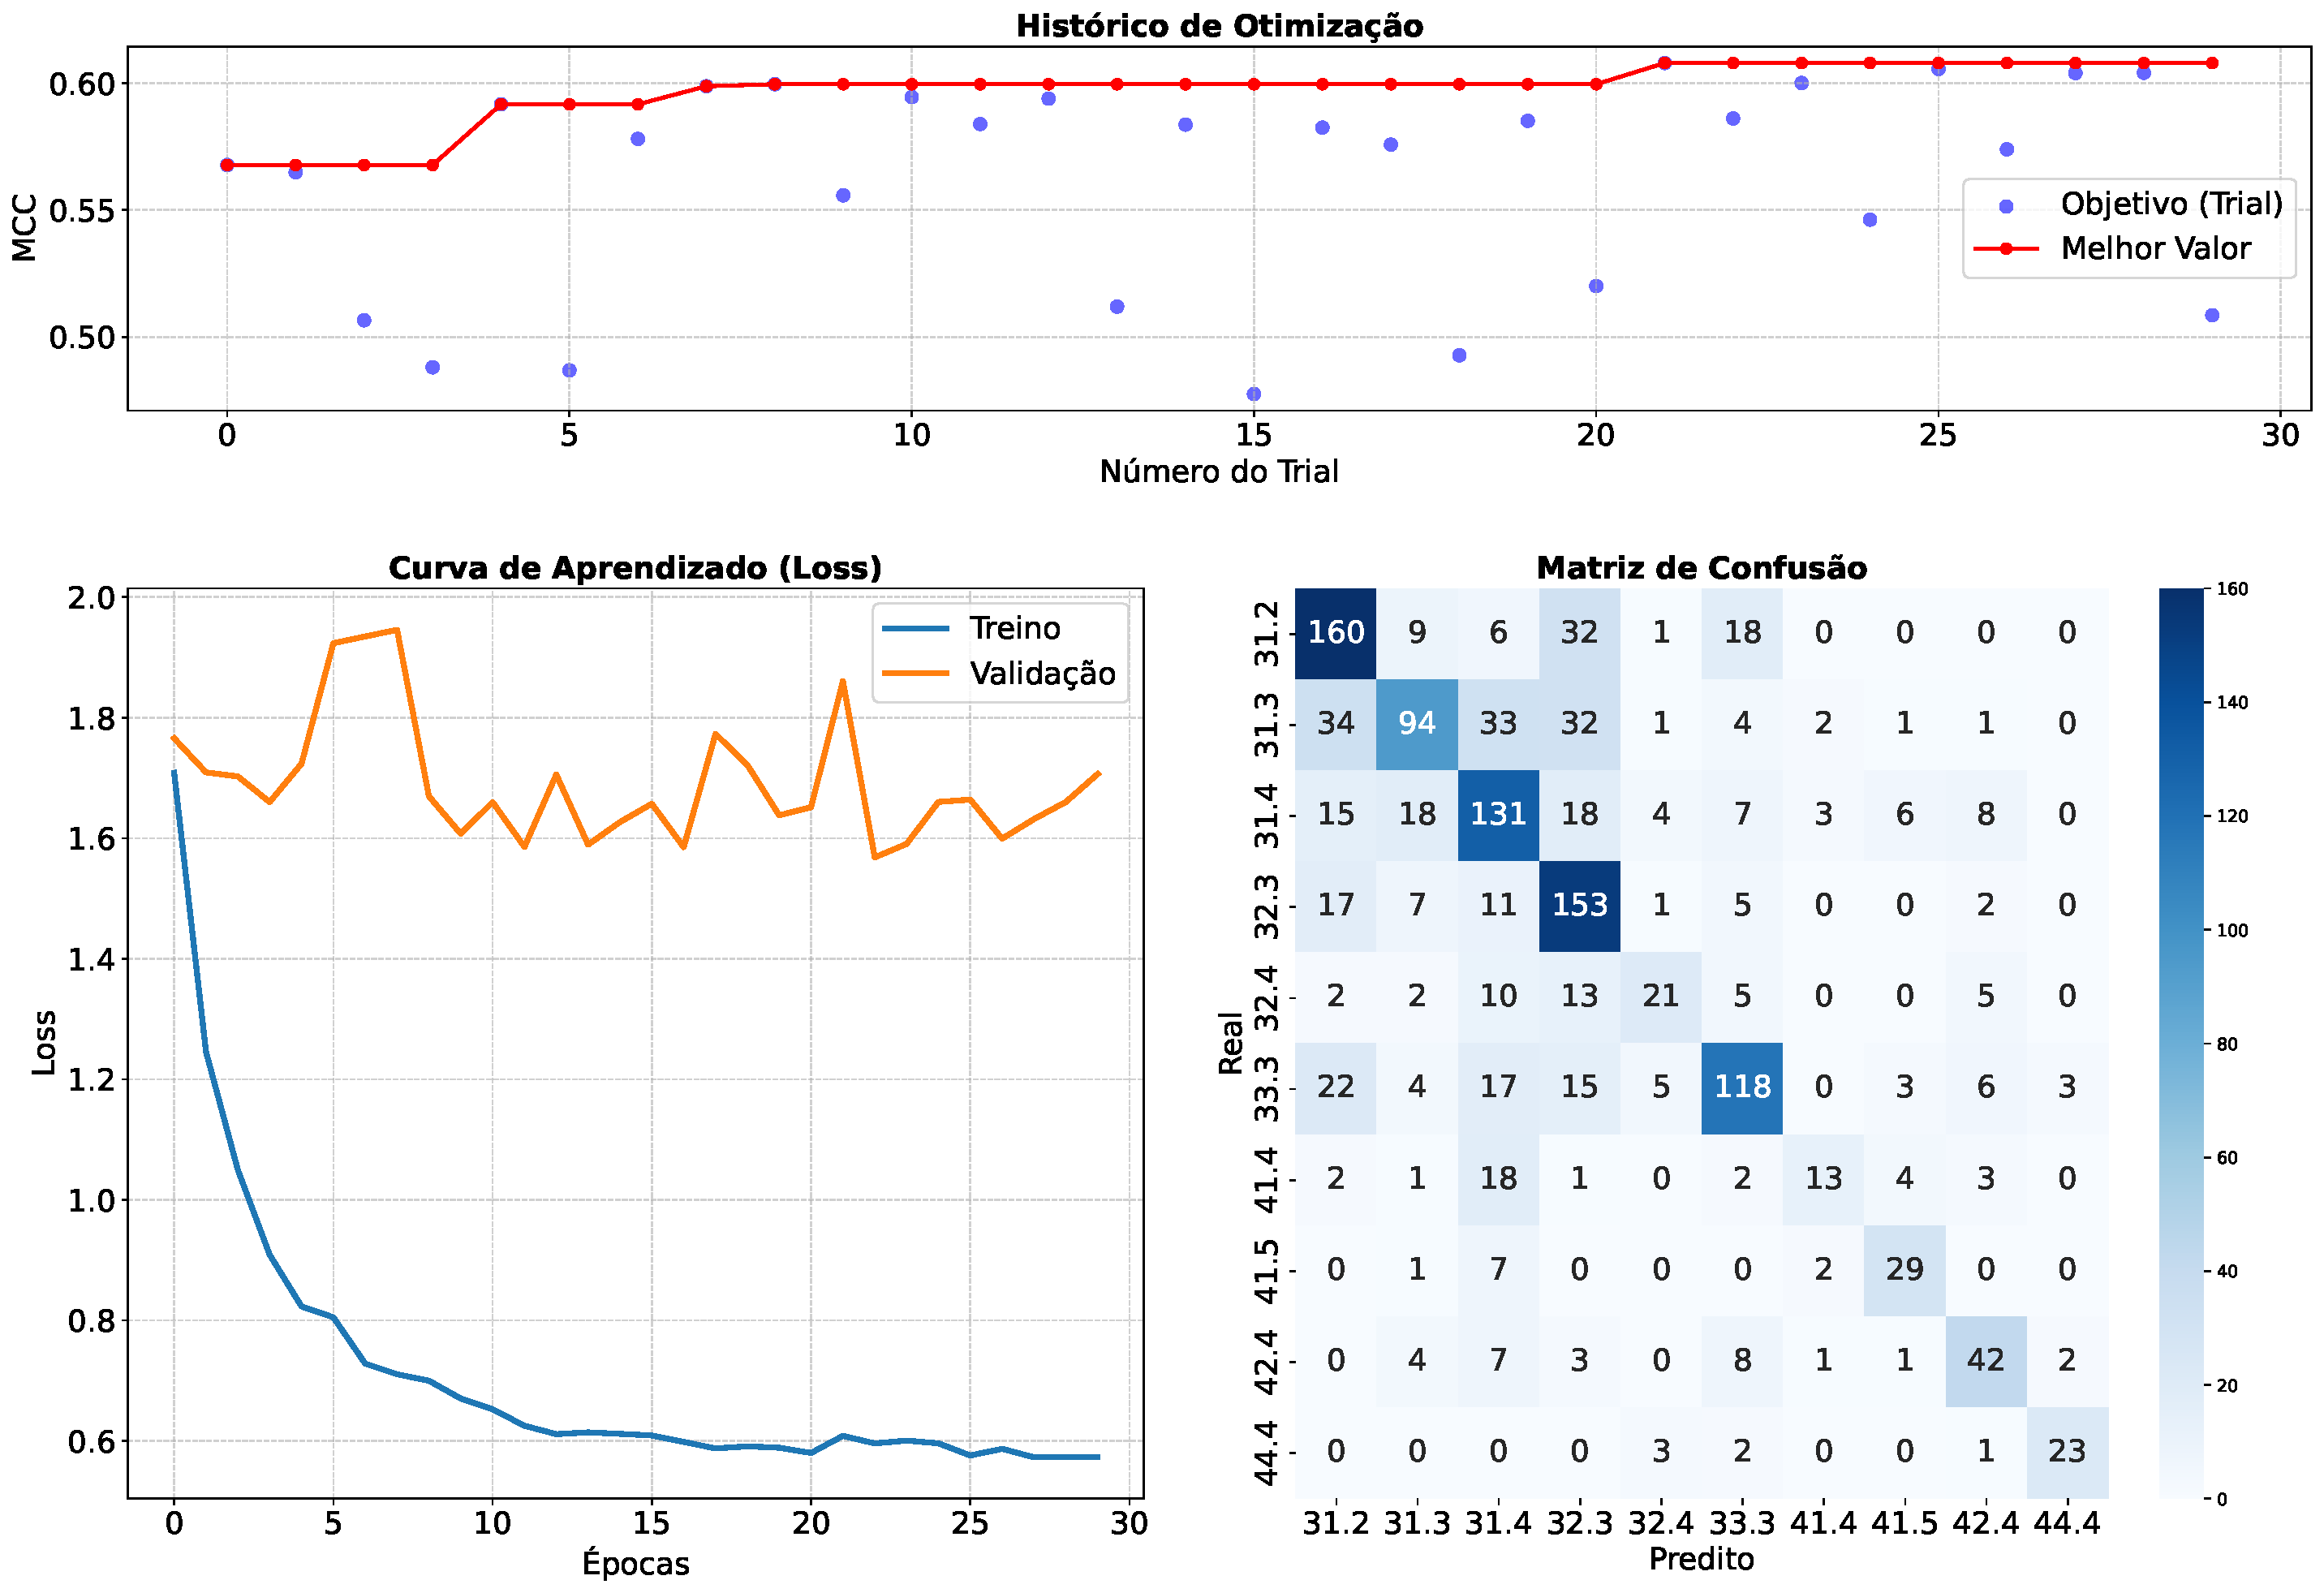
\includegraphics[width=0.85\textwidth]{tex/appendix/experiments/efficientnet_v9_AM_opt_aug/dashboard_consolidado.pdf}
        \caption{Histórico de Otimização, Curvas de Aprendizado e Matriz de Confusão - efficientnet\_v9\_AM\_opt\_aug}
    \end{figure}
\end{minipage}
\clearpage
